\documentclass[multi=my,crop, margin=1pt]{standalone}
\usepackage{color,xcolor}
\usepackage{tikz-qtree, tikz}
\usepackage[utf8]{inputenc} 
\usetikzlibrary{decorations.pathreplacing,arrows,shapes,positioning,shadows,calc}
\usetikzlibrary{decorations, decorations.text,backgrounds}
\usetikzlibrary{positioning,arrows,patterns,decorations.markings,arrows.meta}

\usepackage{fontspec}
\setmainfont{Fira Sans} 
\setsansfont{Fira Sans Light}

\begin{document}


 %%%%%%%%%%%%%%%%%%%

% Opera 1
\begin{my}
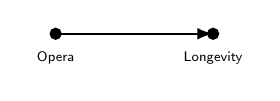
\begin{tikzpicture}[node distance=2cm, font=\sffamily\tiny]
  \draw[-{Latex[length=2mm]},thick] (0,0)--(2,0);
    \foreach \x/\name in {0/Opera,2/Longevity}{\path[draw, fill=black] (\x,0) circle[radius=2pt] node [below=1 mm, black] {\name};}
\end{tikzpicture}
 \end{my}
 
 % Opera 2
 \begin{my}
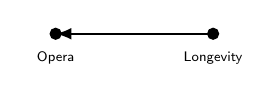
\begin{tikzpicture}[node distance=2cm, font=\sffamily\tiny]
       \draw[-{Latex[length=2mm]},thick] (2,0)--(0,0);
        \foreach \x/\name in {0/Opera,2/Longevity}{\path[draw, fill=black] (\x,0) circle[radius=2pt] node [below=1 mm, black] {\name};}
\end{tikzpicture}
 \end{my}
 
 % Opera 3
\begin{my}
 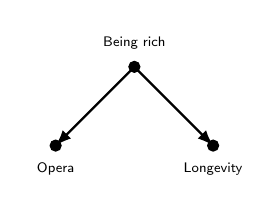
\begin{tikzpicture}[node distance=2cm, font=\sffamily\tiny]
        \foreach \x/\name in {0/Opera,2/Longevity}{\path[draw, fill=black] (\x,0) circle[radius=2pt] node [below=1 mm, black] {\name};}
        \foreach \x/\name in {1/Being rich}{\path[draw, fill=black] (\x,1) circle[radius=2pt] node [above=1 mm, black] {\name};}
       \draw[-{Latex[length=2mm]},thick] (1,1) -- (0,0);
       \draw[-{Latex[length=2mm]},thick] (1,1) -- (2,0);
\end{tikzpicture}
\end{my}
  
 % Opera 4
\begin{my}
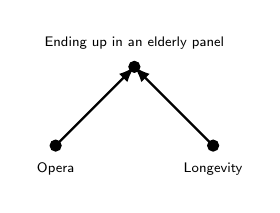
\begin{tikzpicture}[node distance=2cm, font=\sffamily\tiny]
        \foreach \x/\name in {0/Opera,2/Longevity}{\path[draw, fill=black] (\x,0) circle[radius=2pt] node [below=1 mm, black] {\name};}
        \foreach \x/\name in {1/Ending up in an elderly panel}{\path[draw, fill=black] (\x,1) circle[radius=2pt] node [above=1 mm, black] {\name};}
       \draw[-{Latex[length=2mm]},thick] (0,0) -- (1,1);
       \draw[-{Latex[length=2mm]},thick] (2,0) -- (1,1);
\end{tikzpicture}
\end{my} 

% Randomization
\begin{my}
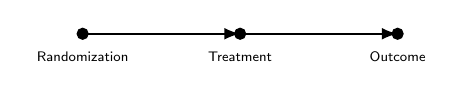
\begin{tikzpicture}[node distance=2cm, font=\sffamily\tiny]
       \draw[-{Latex[length=2mm]},thick] (0,0) -- (2,0) edge (4,0);
        \foreach \x/\name in {0/Randomization,2/Treatment,4/Outcome}{\path[draw, fill=black] (\x,0) circle[radius=2pt] node [below=1 mm, black] {\name};}
\end{tikzpicture}
\end{my}
 
 %%%%%%%%%%%%%%%%%%%
 
 % Nodes
\begin{my}
      \begin{tikzpicture}
        \foreach \x/\name in {0/D,2/Y}{ \path[draw, fill=black] (\x,0) circle[radius=2pt] node [below=1 mm, black] {\name};}
    \end{tikzpicture}
\end{my}
 
 % Arrows
\begin{my}
      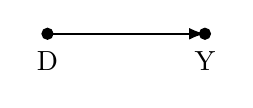
\begin{tikzpicture}
       \draw[-{Latex[length=2mm]},thick] (0,0)--(2,0);
        \foreach \x/\name in {0/D,2/Y}{\path[draw, fill=black] (\x,0) circle[radius=2pt] node [below=1 mm, black] {\name};}
    \end{tikzpicture}
\end{my}
 
 % Endogeneity
\begin{my}
      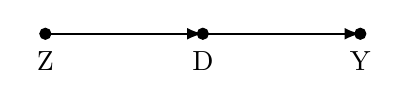
\begin{tikzpicture}
       \draw[-{Latex[length=2mm]},thick] (0,0) -- (2,0) edge (4,0);
        \foreach \x/\name in {0/Z,2/D,4/Y}{\path[draw, fill=black] (\x,0) circle[radius=2pt] node [below=1 mm, black] {\name};}
    \end{tikzpicture}
\end{my}
 
 % Paths
\begin{my}
      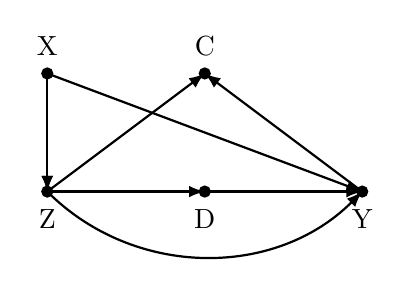
\begin{tikzpicture}
        \foreach \x/\name in {0/Z,2/D,4/Y}{\path[draw, fill=black] (\x,0) circle[radius=2pt] node [below=1 mm, black] {\name};}
        \foreach \x/\name in {0/X,2/C}{\path[draw, fill=black] (\x,1.5) circle[radius=2pt] node [above=1 mm, black] {\name};}
       \draw[-{Latex[length=2mm]},thick] (0,0) -- (2,0) edge (4,0);
       \draw[-{Latex[length=2mm]},thick] (0,1.5) -- (0,0);
       \draw[-{Latex[length=2mm]},thick] (0,0) -- (2,1.5);
       \draw[-{Latex[length=2mm]},thick] (0,1.5) -- (4,0);
       \draw[-{Latex[length=2mm]},thick] (4,0) -- (2,1.5);
       \draw[-{Latex[length=2mm]},thick] (0,1) -- (0,0) edge[bend right=45] (4,0);
    \end{tikzpicture}
\end{my}
 
 % Fork
\begin{my}
      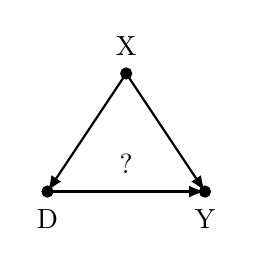
\begin{tikzpicture}
        \foreach \x/\name in {0/D,2/Y}{\path[draw, fill=black] (\x,0) circle[radius=2pt] node [below=1 mm, black] {\name};}
        \foreach \x/\name in {1/X}{\path[draw, fill=black] (\x,1.5) circle[radius=2pt] node [above=1 mm, black] {\name};}
       \draw[-{Latex[length=2mm]},thick] (0,0) -- (2,0);
       \draw[-{Latex[length=2mm]},thick] (1,1.5) -- (0,0);
       \draw[-{Latex[length=2mm]},thick] (1,1.5) -- (2,0);
       \node[above=1mm, black, thick] at (1, 0) {?};
    \end{tikzpicture}
\end{my}

% Mediator
\begin{my}
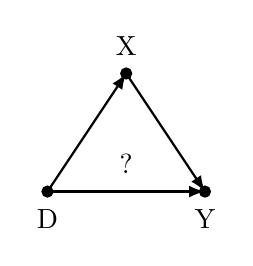
\begin{tikzpicture}
        \foreach \x/\name in {0/D,2/Y}{\path[draw, fill=black] (\x,0) circle[radius=2pt] node [below=1 mm, black] {\name};}
        \foreach \x/\name in {1/X}{\path[draw, fill=black] (\x,1.5) circle[radius=2pt] node [above=1 mm, black] {\name};}
       \draw[-{Latex[length=2mm]},thick] (0,0) -- (2,0);
       \draw[-{Latex[length=2mm]},thick] (0,0) -- (1,1.5);
       \draw[-{Latex[length=2mm]},thick] (1,1.5) -- (2,0);
       \node[above=1mm, black, thick] at (1, 0) {?};
    \end{tikzpicture}
 \end{my}
 
 % Collider
 \begin{my}
 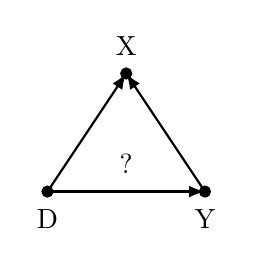
\begin{tikzpicture}
        \foreach \x/\name in {0/D,2/Y}{\path[draw, fill=black] (\x,0) circle[radius=2pt] node [below=1 mm, black] {\name};}
        \foreach \x/\name in {1/X}{\path[draw, fill=black] (\x,1.5) circle[radius=2pt] node [above=1 mm, black] {\name};}
       \draw[-{Latex[length=2mm]},thick] (0,0) -- (2,0);
       \draw[-{Latex[length=2mm]},thick] (0,0) -- (1,1.5);
       \draw[-{Latex[length=2mm]},thick] (2,0) -- (1,1.5);
       \node[above=1mm, black, thick] at (1, 0) {?};
    \end{tikzpicture}
 \end{my}
 
 % Confounder example
 \begin{my}
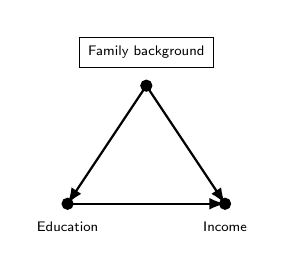
\begin{tikzpicture}[node distance=2cm, font=\sffamily\tiny]
        \foreach \x/\name in {0/Education,2/Income}{\path[draw, fill=black] (\x,0) circle[radius=2pt] node [below=1 mm, black] {\name};}
        \foreach \x/\name in {1/\fbox{Family background}}{\path[draw, fill=black] (\x,1.5) circle[radius=2pt] node [above=1 mm, black] {\name};}
       \draw[-{Latex[length=2mm]},thick] (0,0) -- (2,0);
       \draw[-{Latex[length=2mm]},thick] (1,1.5) -- (0,0);
       \draw[-{Latex[length=2mm]},thick] (1,1.5) -- (2,0);
    \end{tikzpicture}
 \end{my}
 
 % Confounder example 2
\begin{my}
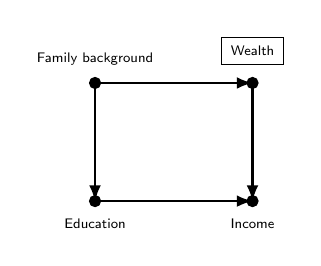
\begin{tikzpicture}[node distance=2cm, font=\sffamily\tiny]
        \foreach \x/\name in {0/Education,2/Income}{\path[draw, fill=black] (\x,0) circle[radius=2pt] node [below=1 mm, black] {\name};}
        \foreach \x/\name in {0/Family background,2/\fbox{Wealth}}{\path[draw, fill=black] (\x,1.5) circle[radius=2pt] node [above=1 mm, black] {\name};}
       \draw[-{Latex[length=2mm]},thick] (0,0) -- (2,0);
       \draw[-{Latex[length=2mm]},thick] (0,1.5) -- (0,0);
       \draw[-{Latex[length=2mm]},thick] (0,1.5) -- (2,1.5);
       \draw[-{Latex[length=2mm]},thick] (2,1.5) -- (2,0);
    \end{tikzpicture}
 \end{my}
 
 % Mediator example
 \begin{my}
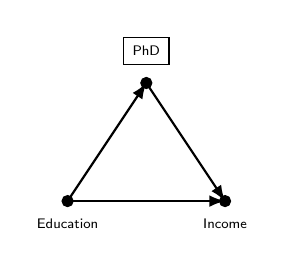
\begin{tikzpicture}[node distance=2cm, font=\sffamily\tiny]
        \foreach \x/\name in {0/Education,2/Income}{\path[draw, fill=black] (\x,0) circle[radius=2pt] node [below=1 mm, black] {\name};}
        \foreach \x/\name in {1/\fbox{PhD}}{\path[draw, fill=black] (\x,1.5) circle[radius=2pt] node [above=1 mm, black] {\name};}
       \draw[-{Latex[length=2mm]},thick] (0,0) -- (2,0);
       \draw[-{Latex[length=2mm]},thick] (0,0) -- (1,1.5);
       \draw[-{Latex[length=2mm]},thick] (1,1.5) -- (2,0);
    \end{tikzpicture}
 \end{my}
 
 % Mediator example 2
\begin{my}
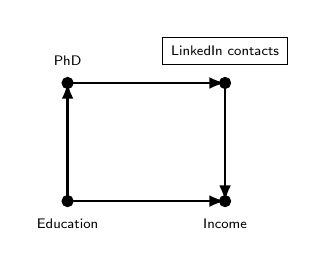
\begin{tikzpicture}[node distance=2cm, font=\sffamily\tiny]
        \foreach \x/\name in {0/Education,2/Income}{\path[draw, fill=black] (\x,0) circle[radius=2pt] node [below=1 mm, black] {\name};}
        \foreach \x/\name in {0/PhD,2/\fbox{LinkedIn contacts}}{\path[draw, fill=black] (\x,1.5) circle[radius=2pt] node [above=1 mm, black] {\name};}
       \draw[-{Latex[length=2mm]},thick] (0,0) -- (2,0);
       \draw[-{Latex[length=2mm]},thick] (0,0) -- (0,1.5) ;
       \draw[-{Latex[length=2mm]},thick] (0,1.5) -- (2,1.5);
       \draw[-{Latex[length=2mm]},thick] (2,1.5) -- (2,0);
    \end{tikzpicture}
 \end{my}
 
 % More complex DAG
\begin{my}
       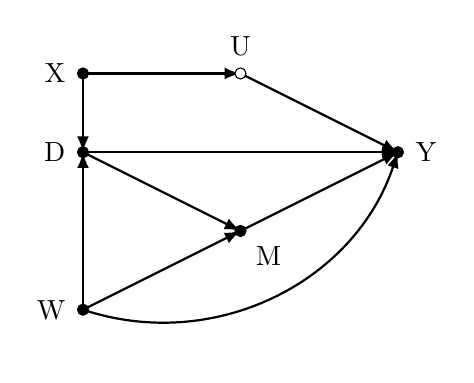
\begin{tikzpicture}
       \draw[-{Latex[length=2mm]},thick] (0,1) -- (0,0);
       \draw[-{Latex[length=2mm]},thick] (0,1) -- (2,1);
       \draw[-{Latex[length=2mm]},thick] (0,0) -- (4,0);
       \draw[-{Latex[length=2mm]},thick] (2,1) -- (4,0);
       \draw[-{Latex[length=2mm]},thick] (0,0) -- (2,-1);
       \draw[-{Latex[length=2mm]},thick] (2,-1) -- (4,0);
       \draw[-{Latex[length=2mm]},thick] (0,-2) -- (0,0);
       \draw[-{Latex[length=2mm]},thick] (0,-2) -- (2,-1);
       \path[-{Latex[length=2mm]},thick] (0,-2) edge[bend right=45] (4,0);
        \foreach \x/\name in {0/D}{\path[draw, fill=black] (\x,0) circle[radius=2pt] node [left=1 mm, black] {\name};}
        \foreach \x/\name in {4/Y}{\path[draw, fill=black] (\x,0) circle[radius=2pt] node [right=1 mm, black] {\name};}
        \foreach \x/\name in {2/M}{\path[draw, fill=black] (\x,-1) circle[radius=2pt] node [below right=1 mm, black] {\name};}
        \foreach \x/\name in {0/W}{\path[draw, fill=black] (\x,-2) circle[radius=2pt] node [left=1 mm, black] {\name};}
        \foreach \x/\name in {0/X}{\path[draw, fill=black] (\x,1) circle[radius=2pt] node [left=1 mm, black] {\name};}
        \foreach \x/\name in {2/U}{\path[draw, fill=white] (\x,1) circle[radius=2pt] node [above=1 mm, black] {\name};}
    \end{tikzpicture}
 \end{my}
 
 % Collider bias
\begin{my}
       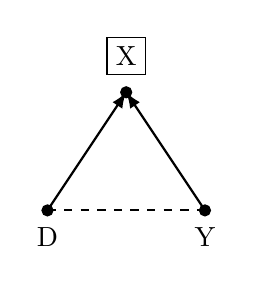
\begin{tikzpicture}
        \foreach \x/\name in {0/D,2/Y}{\path[draw, fill=black] (\x,0) circle[radius=2pt] node [below=1 mm, black] {\name};}
        \foreach \x/\name in {1/\fbox{X}}{\path[draw, fill=black] (\x,1.5) circle[radius=2pt] node [above=1 mm, black] {\name};}
       \draw[dashed,thick] (0,0) -- (2,0);
       \draw[-{Latex[length=2mm]},thick] (0,0) -- (1,1.5);
       \draw[-{Latex[length=2mm]},thick] (2,0) -- (1,1.5);
    \end{tikzpicture}
 \end{my}
 
  % Collider bias: example
\begin{my}
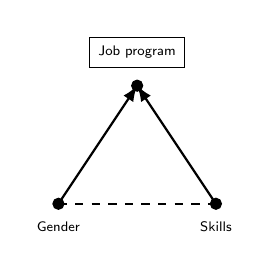
\begin{tikzpicture}[node distance=2cm, font=\sffamily\tiny]
        \foreach \x/\name in {0/Gender,2/Skills}{\path[draw, fill=black] (\x,0) circle[radius=2pt] node [below=1 mm, black] {\name};}
        \foreach \x/\name in {1/\fbox{Job program}}{\path[draw, fill=black] (\x,1.5) circle[radius=2pt] node [above=1 mm, black] {\name};}
       \draw[dashed,thick] (0,0) -- (2,0);
       \draw[-{Latex[length=2mm]},thick] (0,0) -- (1,1.5);
       \draw[-{Latex[length=2mm]},thick] (2,0) -- (1,1.5);
    \end{tikzpicture}
 \end{my}
 
% Collider bias: example 2
\begin{my}
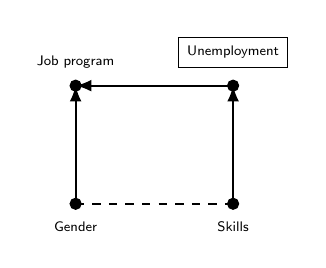
\begin{tikzpicture}[node distance=2cm, font=\sffamily\tiny]
        \foreach \x/\name in {0/Gender,2/Skills}{\path[draw, fill=black] (\x,0) circle[radius=2pt] node [below=1 mm, black] {\name};}
        \foreach \x/\name in {0/Job program,2/\fbox{Unemployment}}{\path[draw, fill=black] (\x,1.5) circle[radius=2pt] node [above=1 mm, black] {\name};}
       \draw[dashed,thick] (0,0) -- (2,0);
       \draw[-{Latex[length=2mm]},thick] (0,0) -- (0,1.5) ;
       \draw[-{Latex[length=2mm]},thick] (2,1.5) -- (0,1.5);
       \draw[-{Latex[length=2mm]},thick] (2,0) --(2,1.5);
    \end{tikzpicture}
 \end{my}
 
 % Opera 1
\begin{my}
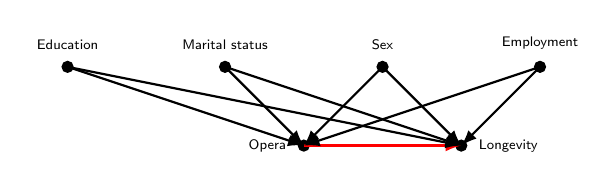
\begin{tikzpicture}[node distance=2cm, font=\sffamily\tiny]
         \path[draw, fill=black] (0,0) circle[radius=2pt] node [left=1 mm, black] {Opera};
         \path[draw, fill=black] (2,0) circle[radius=2pt] node [right=1 mm, black] {Longevity};
                  \draw[-{Latex[length=2mm]},thick, red] (0,0) -- (2,0);
                  	\foreach \x/\name in {-3/Education,-1/Marital status,1/Sex,3/Employment}{\path[draw, fill=black] (\x,1) circle[radius=2pt] node [above=1 mm, black] {\name};}
	\foreach \x in {-3,-1,1,3}\draw[-{Latex[length=2mm]},thick] (\x,1) -- (0,0);
       \foreach \x in {-3,-1,1,3}\draw[-{Latex[length=2mm]},thick] (\x,1) -- (2,0);
\end{tikzpicture}
 \end{my}
 
 % Opera 2
\begin{my}
 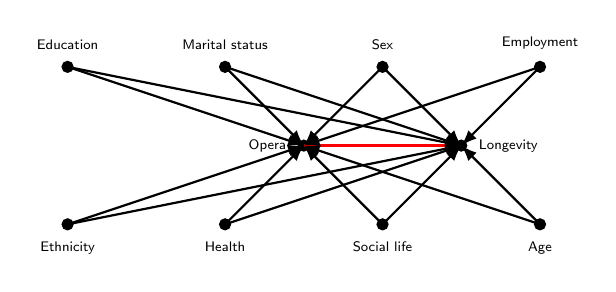
\begin{tikzpicture}[node distance=2cm, font=\sffamily\tiny]
         \path[draw, fill=black] (0,0) circle[radius=2pt] node [left=1 mm, black] {Opera};
         \path[draw, fill=black] (2,0) circle[radius=2pt] node [right=1 mm, black] {Longevity};
         \draw[-{Latex[length=2mm]},thick, red] (0,0) -- (2,0);
	\foreach \x/\name in {-3/Education,-1/Marital status,1/Sex,3/Employment}{\path[draw, fill=black] (\x,1) circle[radius=2pt] node [above=1 mm, black] {\name};}
	\foreach \x in {-3,-1,1,3}\draw[-{Latex[length=2mm]},thick] (\x,1) -- (0,0);
       \foreach \x in {-3,-1,1,3}\draw[-{Latex[length=2mm]},thick] (\x,1) -- (2,0);
       \foreach \x/\name in {-3/Ethnicity,-1/Health,1/Social life,3/Age}{\path[draw, fill=black] (\x,-1) circle[radius=2pt] node [below=1 mm, black] {\name};}
       \foreach \x in {-3,-1,1,3}\draw[-{Latex[length=2mm]},thick] (\x,-1) -- (0,0);
       \foreach \x in {-3,-1,1,3}\draw[-{Latex[length=2mm]},thick] (\x,-1) -- (2,0);
\end{tikzpicture}
 \end{my}
 

 \begin{my}
      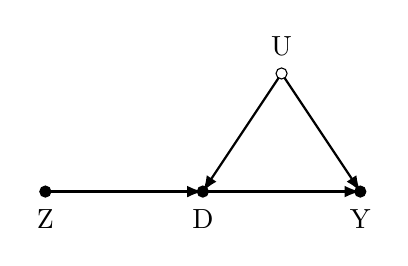
\begin{tikzpicture}
               \draw[-{Latex[length=2mm]},thick] (-2,0) -- (0,0);
       \draw[-{Latex[length=2mm]},thick] (0,0) -- (2,0);
       \draw[-{Latex[length=2mm]},thick] (1,1.5) -- (0,0);
       \draw[-{Latex[length=2mm]},thick] (1,1.5) -- (2,0);
        \foreach \x/\name in {-2/Z}{\path[draw, fill=black] (\x,0) circle[radius=2pt] node [below=1 mm, black] {\name};}
        \foreach \x/\name in {0/D,2/Y}{\path[draw, fill=black] (\x,0) circle[radius=2pt] node [below=1 mm, black] {\name};}
        \foreach \x/\name in {1/U}{\path[draw, fill=white] (\x,1.5) circle[radius=2pt] node [above=1 mm, black] {\name};}
    \end{tikzpicture}
 \end{my}
 
 % Musical genres and death
 \begin{my}
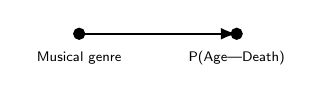
\begin{tikzpicture}[node distance=2cm, font=\sffamily\tiny]
  \draw[-{Latex[length=2mm]},thick] (0,0)--(2,0);
    \foreach \x/\name in {0/Musical genre,2/P(Age|Death)}{\path[draw, fill=black] (\x,0) circle[radius=2pt] node [below=1 mm, black] {\name};}
\end{tikzpicture}
 \end{my}
 
  % Musical genres and death 2
 \begin{my}
 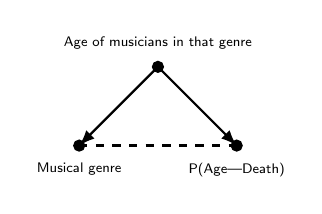
\begin{tikzpicture}[node distance=2cm, font=\sffamily\tiny]
        \foreach \x/\name in {0/Musical genre,2/P(Age|Death)}{\path[draw, fill=black] (\x,0) circle[radius=2pt] node [below=1 mm, black] {\name};}
        \foreach \x/\name in {1/Age of musicians in that genre}{\path[draw, fill=black] (\x,1) circle[radius=2pt] node [above=1 mm, black] {\name};}
       \draw[-{Latex[length=2mm]},thick] (1,1) -- (0,0);
       \draw[-{Latex[length=2mm]},thick] (1,1) -- (2,0);
              \draw[dashed,thick] (0,0) -- (2,0);
\end{tikzpicture}
 \end{my}
 
 \begin{my}

 \end{my}
 
 \begin{my}

 \end{my}
 
 \begin{my}

 \end{my}
 
 \begin{my}

 \end{my}
 
 \begin{my}

 \end{my}
 
 
\end{document}





